%%%%%%%%%%%%%%%%%%%%%%%%%%%%%%%%%%%%%%%%%%%%%%%%%%%%%%%%%%%%%%%%%
\chapter{GENERALIZED DIFFERENTIAL QUADRATURE METHOD}\label{ch:fp}
%%%%%%%%%%%%%%%%%%%%%%%%%%%%%%%%%%%%%%%%%%%%%%%%%%%%%%%%%%%%%%%%%

\section{Motivation and Historical Advance}

Solving differential equations has always been a challenge either they are ordinary or partial. When there is no analytical solution, numerical techniques are referred to and thanks to the exponential increase in the capacity of processing power in processors, it is possible to have solutions to a variety of complicated problems with an satisfactory accuracy. But still, for some specific applications, such as embedded systems, computational power might be limited which requires some intelligent techniques for discretizing the equations to have fast and accurate solutions. Most of the times, there exists a trade - off between accuracy and computation time, so the balance would also be a function of the requirements of the system in the focus of interest. Solution of differential equations might be necessary for optimization and optimal control problems, making it a crucial step to complete starting from the design step to eventually controlling it during its mission execution.  

For the problems whose governing partial differential equations are difficult or not possible to be solved in closed-form, approximate solutions are turned to. Basically, approximate solutions are the relations between the derivatives in the partial differential equation and the functional values at certain discrete points(grid points or mesh points). This relation between those two is attained by numerical discretization and coins the terms for the solutions as numerical solutions.

Numerical discretization techniques are not new or lacking, a wide variety of options are available in the literature. Each possess some advantage over the others. To name a few are the finite difference method, finite element method under low order methods whereas spectral and pseudospectral methods as global methods. Finite difference method relies on Taylor series expansion or polynomial approximation while finite element method is based on variational principle or the weighted residuals principle. Spectral methods use a developed version of method of weighted residuals which heavily rely on base and weighting functions. The similarity that both finite element and spectral methods use of set of base functions differentiate in their choices of base functions.

Most of the engineering problems can be solved via low order methods such as finite element, finite difference, and finite volume, for a large number of grid points. The necessity to use a larger set of grip points to have satisfactorily accurate solutions might be a burden for applications where solutions for the whole physical domain is not really necessary, i.e the user only needs the solutions for a specific part of the domain.

Accurate solutions with less number of grids is of concern also since it requires less computational need which is required for a variety of disciplines. With such a goal, Differential Quadrature Method(DQM) has been offered by Richard Bellmann and his colleagues in 1971. They were in search to have satisfactorily precise solutions with a small number of grids. 

Differential quadrature relies on the calculation of a partial derivative of a function with respect to a coordinate direction by a linear weighted sum of all evaluated function values at all the grid points along the same direction. It is inspired from integral quadrature.

Integral quadrature is the evaluation of integral $\int_{a}^{b} f(x)dx$ over a finite internal $[a,b]$. When it is not possible to find an explicit solution for $F$ such that $\frac{dF}{dx}=f$, the knowledge of $f$ at grid points can be used to approximate the integral. This integral also can be represented as the area under the curve represented by $f(x)$ as seen in Figure~\ref{intQuad}. So the idea is to find the approximate value of the integral, the area under the curve can be calculated approximately such as

\begin{figure}
\centerline{\psfig{figure=figures/intQuad.eps,width=4.3in}}
\vspace*{6mm}
\caption{Integral of $f(x)$ over an interval.}
\label{intQuad} 
\end{figure}

\begin{equation} \label{integralQuadrature}
\int_{a}^b f(x)dx = w_1 f_1 + w_2 f_2 + ... + w_n f_n = \sum_{k=1}^n w_k f_k
\end{equation}

where $w_1, w_2, ..., w_n$ are the weighting coefficients, $f_1, f_2, f, ..., f_n$ are the functional values at grid points $a =x_1, x_2, ..., x_n = b$ and Equation \eqref{integralQuadrature} is the equation of integral quadrature. The choice of these discrete grid points vary depending on the problem.

This idea of calculating the integral of a function inspired the differential quadrature. Bellmann suggested that the 1st order derivative of a function $f(x)$ with respect to $x$ evaluated at a grid point $x_i$ can be approximated as a linear sum of all the functional values evaluated at all grid points along this dimension. For one-dimensional problem as given in Figure~\ref{oneDimGrid} the 1st order derivative of a function $f(x)$ with respect to $x$ evaluated at a grid point $x_i$ can be written as

\begin{equation} \label{firstOrderDerivative}
f_x(x_i)= \frac{df}{dx} \biggr\rvert_{x_i} = \sum_{j=1}^N a_{ij} \cdot f(x_j), \quad for \ i = 1,2, ...,N
\end{equation}

where $a_{ij}$ are the weighting coefficients, $N$ is the number of grids. The key procedure of DQM is to select the weighting coefficients.

Differential Quadrature, inspired by integral quadrature, is a powerful technique to approximate the derivatives of a function at a point as a weighted linear sum of all the functional values at discrete points along the derivation direction. To generalize, in DQM, the ${{n}^{th}}$ order derivative of a single variable function $u\left( y \right)$ can be approximated as given in \eqref{nthOrderDerivative}.

\begin{equation} \label{nthOrderDerivative}
{{u}^{(n)}}({{y}_{i}})=\sum\limits_{j=1}^{N}{c_{ij}^{(n)}}u({{y}_{j}})\text{ }\quad i=1,2,\ldots ,N
\end{equation}

where $c_{ij}^{\left( n \right)}$  are the weighting coefficients for the ${{n}^{th}}$ order derivative, and N is the number of grids. The challenging step in utilization of DQM is the calculation of weighting coefficients. Bellmann offered two methods to calculate the first order coefficients \cite{BellmanDQM}. To show how, let's specialize in the first order derivative case rather than the general $n^{th}$ order case. For that write again the first order derivative approximation, but this time indicating that this is the first derivative as

\begin{equation} \label{firstOrderDerivative2}
f_x^{(1)}(x_i)= \sum_{j=1}^N a_{ij} \cdot f(x_j), \quad for \ i = 1,2, ...,N
\end{equation}

\begin{figure}
\centerline{\psfig{figure=figures/oneDimGrid.eps,width=4.3in}}
\vspace*{6mm}
\caption{One-dimensional problem gridding example.}
\label{oneDimGrid} 
\end{figure}

Both of Bellmann's methods to calculate the weighting coefficients are based on test functions which defer from one to the other. In the first method, the $N$ test functions are selected as

\begin{equation} \label{testFuncFirstMethod}
g_k(x)= x^k, \quad for \ k = 0,2, ...,N-1
\end{equation}

since $i$ and $j$ is varied from $1$ to $N$ as seen from Equ. \eqref{firstOrderDerivative2}, the number of weighting coefficients $a_{ij}$ is $NxN$. When these N test functions given in Equ. \eqref{testFuncFirstMethod} are applied to $N$ grid points, $NxN$ algebraic equations 

\begin{align}
\begin{split}
&\sum_{j=1}^N a_{ij} =0\\
&\sum_{j=1}^N a_{ij} \cdot x_j =0 \\
&\sum_{j=1}^N a_{ij} \cdot x_j^k = k \cdot x_i^{k-1}, \quad k = 2,3, ..., N-1 \\
&for \quad i = 1,2, ..., N
\end{split}
\end{align}

are obtained to solve for $NxN$ weighting coefficients $a_{ij}$. The system of equations form a Vandermonde matrix and has a unique solution. But when $N$ gets larger the matrix becomes ill-conditioned and inversion is challenging. In its applications, the number of grids is restricted to be less than 13. Although the coordinates of the grid points are chosen arbitrarily, the restriction on the number of grids widely narrowed its applications. 

In the second method, the test functions used are 

\begin{equation} \label{testFuncSecondMethod}
g_k(x)= \frac{L_N(x)}{(x-x_k)L_N^{(1)}(x_k)}, \quad for \ k = 1,2, ...,N
\end{equation}

where $L_N(x)$ is the Legendre polynomial of degree $N$ and $L_N^{1}(x)$ is its first derivative.When $x_k$ is chosen to be the roots of the Legendre polynomial and Equ. \eqref{testFuncSecondMethod} is written at all grid points, an algebraic relations is attained to calculate the weighting coefficients.

\begin{align}
\begin{split}
a_{ij} &= \frac{L_N^{(1)}(x_i)}{(x_i-x_j)L_N^{(1)}(x_j)}, \quad for j \neq i \\
a_{ii} &= \frac{1-2x_i}{2x_i(x_i -1)}
\end{split}
\end{align}

Although calculation of weighting coefficients is a simple algebraic formulation, the selection of grid point coordinates are restricted to lie at the Legendre polynomial. 

These drawbacks limited the use of method until a major breakthrough is attained by Shu and Richards \cite{ShuDQM} where all the methods available are generalized under the analysis of a high order polynomial approximation and analysis of a linear vector space. This methodology to calculate the weighting coefficients gives the following formulas given in \eqref{equ21}.

\begin{equation} \label{equ21}
a_{ij}=\left\{ \begin{matrix}
   \frac{{{M}^{\left( 1 \right)}}\left( {{x}_{i}} \right)}{\left( {{x}_{i}}-{{x}_{j}} \right){{M}^{\left( 1 \right)}}\left( {{x}_{j}} \right)} & i\ne j  \\
   -\sum\limits_{j=1,j\ne i}^{N}{a_{ij}} & i=j  \\
\end{matrix} \right.
\end{equation}

where  ${{M}^{\left( 1 \right)}}$  is given by \eqref{equ22}.

\begin{equation} \label{equ22}
{{M}^{\left( 1 \right)}}\left( {{x}_{i}} \right)=\prod\limits_{k=1,k\ne i}^{N}{\left( {{x}_{i}}-{{x}_{k}} \right)}
\end{equation}

This method lets the user to calculate the second and higher order weighting coefficients by a recurrence relationship with arbitrary choice of grid points \cite{ShuDifferential}. To solve the weighting coefficients of higher order derivatives, following recurrence relations given in \eqref{equ23} is used.

\begin{equation} \label{equ23}
w_{ij}^{\left( m \right)}=\left\{ \begin{matrix}
   m\left( w_{ii}^{\left( m-1 \right)}a_{ij}-\frac{w_{ij}^{\left( m-1 \right)}}{\left( {{x}_{i}}-{{x}_{j}} \right)} \right) & i\ne j  \\
   -\sum\limits_{j=1,j\ne i}^{N}{w_{ij}^{\left( m \right)}} & i=j  \\
\end{matrix} \right.
\end{equation}

For the choice of grid points locations, there is a vast number of methods. The two different types of grid distribution selected for numerical study of the problems in this work are equal gridding and Chebyshev-Gauss-Lobatto gridding. Equal gridding ensures that the successive grids have an equal distance in-between. In Chebyshev-Gauss-Lobatto gridding, the grid points are denser at the places closer to the boundaries. The relation giving the coordinates of the grids in Chebyshev-Gauss-Lobatto gridding is given in \eqref{equ24}. 

\begin{equation} \label{equ24}
{{y}_{i}}=\cos \left( \frac{i-1}{N-1}\pi  \right)
\end{equation}

For a better understanding of the DQM, let's apply it to the equation

\begin{equation} \label{DQMApplyExample}
\bigg[\frac{1-y^2}{2} \bigg] \frac{\partial T}{\partial x} -\frac{\partial^2T}{\partial y^2} = 0
\end{equation}

with boundary conditions

\begin{align}
T(0,y)&=0 \label{boundaryCond1} \\
T(x,1)&=1 \label{boundaryCond2} \\
\frac{\partial T}{\partial y}(x,0)&=0 \label{boundaryCond2} 
\end{align}

Using the definition of DQM $n^{th}$ order derivative approximation given in  \eqref{nthOrderDerivative}

\begin{equation} \label{DQMApplyExampleDiscretized}
\bigg[\frac{1-y_j^2}{2} \bigg] \sum_{k=1}^N w_{ik}^{(1)} T_{kj} - \sum_{k=1}^M \bar{w}_{jk}^{(2)} T_{ik} = 0
\end{equation}

and the discretized boundary conditions

\begin{align}
T_{1,j}&=0 \label{discretizedBoundaryCond1} \\
T_{i,M}&=1\label{discretizedBoundaryCond2} \\ 
\frac{\partial T_{i1}}{\partial y}&=0 \label{discretizedBoundaryCond3}
\end{align}

where $i = 1 ... N$ and $j = 1 ... M$. In order to write the set of equations in a matrix format, some of the equations are written explicitly by evaluating some values of $i$ and $j$ such as for $i=1$, $j=1$

\begin{align}
\begin{split} \label{DQMApplyExampleDiscretized2}
 \bigg[\frac{1-y_1^2}{2} \bigg] &\bigg[w_{11}^{(1)} T_{11} + w_{12}^{(1)} T_{21} + \dots + w_{1N}^{(1)} T_{N1}\bigg] \\
-  & \bigg[\bar{w}_{11}^{(2)} T_{11} + \bar{w}_{12}^{(2)} T_{12} + \dots + \bar{w}_{1M}^{(2)} T_{1M}\bigg]=0
\end{split}
\end{align}

and $i=1$, $j=2$

\begin{align}
\begin{split} \label{DQMApplyExampleDiscretized2}
\bigg[\frac{1-y_2^2}{2} \bigg]  & \bigg[w_{11}^{(1)} T_{12} + w_{12}^{(1)} T_{22} + \dots + w_{1N}^{(1)} T_{N2}\bigg] \\
-  & \bigg[\bar{w}_{21}^{(2)} T_{11} + \bar{w}_{22}^{(2)} T_{12} + \dots + \bar{w}_{2M}^{(2)} T_{1M}\bigg]=0
\end{split}
\end{align}

for $i=1$, $j=M$

\begin{align}
\begin{split} \label{DQMApplyExampleDiscretized2}
\bigg[\frac{1-y_M^2}{2} \bigg]  & \bigg[w_{11}^{(1)} T_{1M} + w_{12}^{(1)} T_{2M} + \dots + w_{1N}^{(1)} T_{NM}\bigg]\\
-  & \bigg[\bar{w}_{M1}^{(2)} T_{11} + \bar{w}_{M2}^{(2)} T_{12} + \dots + \bar{w}_{MM}^{(2)} T_{1M}\bigg]=0
\end{split}
\end{align}

and also $i=2$, $j=1$

\begin{align}
\begin{split} \label{DQMApplyExampleDiscretized2}
\bigg[\frac{1-y_1^2}{2} \bigg]  & \bigg[w_{21}^{(1)} T_{11} + w_{22}^{(1)} T_{21} + \dots + w_{2N}^{(1)} T_{N1}\bigg] \\
-  & \bigg[\bar{w}_{11}^{(2)} T_{21} + \bar{w}_{12}^{(2)} T_{22} + \dots + \bar{w}_{1M}^{(2)} T_{2M}\bigg]=0
\end{split}
\end{align}

and also $i=N$, $j=1$

\begin{align}
\begin{split} \label{DQMApplyExampleDiscretized2}
\bigg[\frac{1-y_1^2}{2} \bigg]  & \bigg[w_{N1}^{(1)} T_{11} + w_{N2}^{(1)} T_{21} + \dots + w_{NN}^{(1)} T_{N1}\bigg] \\
-  & \bigg[\bar{w}_{11}^{(2)} T_{N1} + \bar{w}_{12}^{(2)} T_{N2} + \dots + \bar{w}_{1M}^{(2)} T_{NM}\bigg]=0
\end{split}
\end{align}

finally and also $i=N$, $j=M$

\begin{align}
\begin{split} \label{DQMApplyExampleDiscretized2}
\bigg[\frac{1-y_M^2}{2} \bigg]  & \bigg[w_{N1}^{(1)} T_{1M} + w_{N2}^{(1)} T_{2M} + \dots + w_{NN}^{(1)} T_{NM}\bigg] \\
 -  & \bigg[\bar{w}_{M1}^{(2)} T_{N1} + \bar{w}_{M2}^{(2)} T_{N2} + \dots + \bar{w}_{MM}^{(2)} T_{NM}\bigg]=0
\end{split}
\end{align}

These sets of equations are now gathered in matrix form as shown in Figure~\ref{matrixGiantErasedEq} 

\begin{equation} \label{equ24}
\bm{W} \bm{T} = 0
\end{equation}

so that it can be solved via inverting the matrix. Then the boundary conditions are applied to the system of equations by updating the corresponding rows in the matrix representation which shown in Figure~\ref{matrixBoundaries}. This is a linear set of equations which means that the system can be represented in the form \eqref{linearSystem}.

\begin{equation} \label{linearSystem}
\bm{A} \bm{x} = \bm{b}
\end{equation}

To solve for $\bm{x}$, $\bm{A}$ is inverted and multiplied by $\bm{b}$

\begin{equation} \label{solveLinearSystem}
 \bm{x} = \bm{A}^{-1} \bm{b}
\end{equation}

If the system can not be represented in such a form, than it can not be solved via inverting the matrix. For nonlinear problems, after discretization via DQM, some other method, such as Newton-Raphson should be referred for the solution of system of equations.

\begin{landscape}
\thispagestyle{empty}
\begin{figure}
\begin{center}
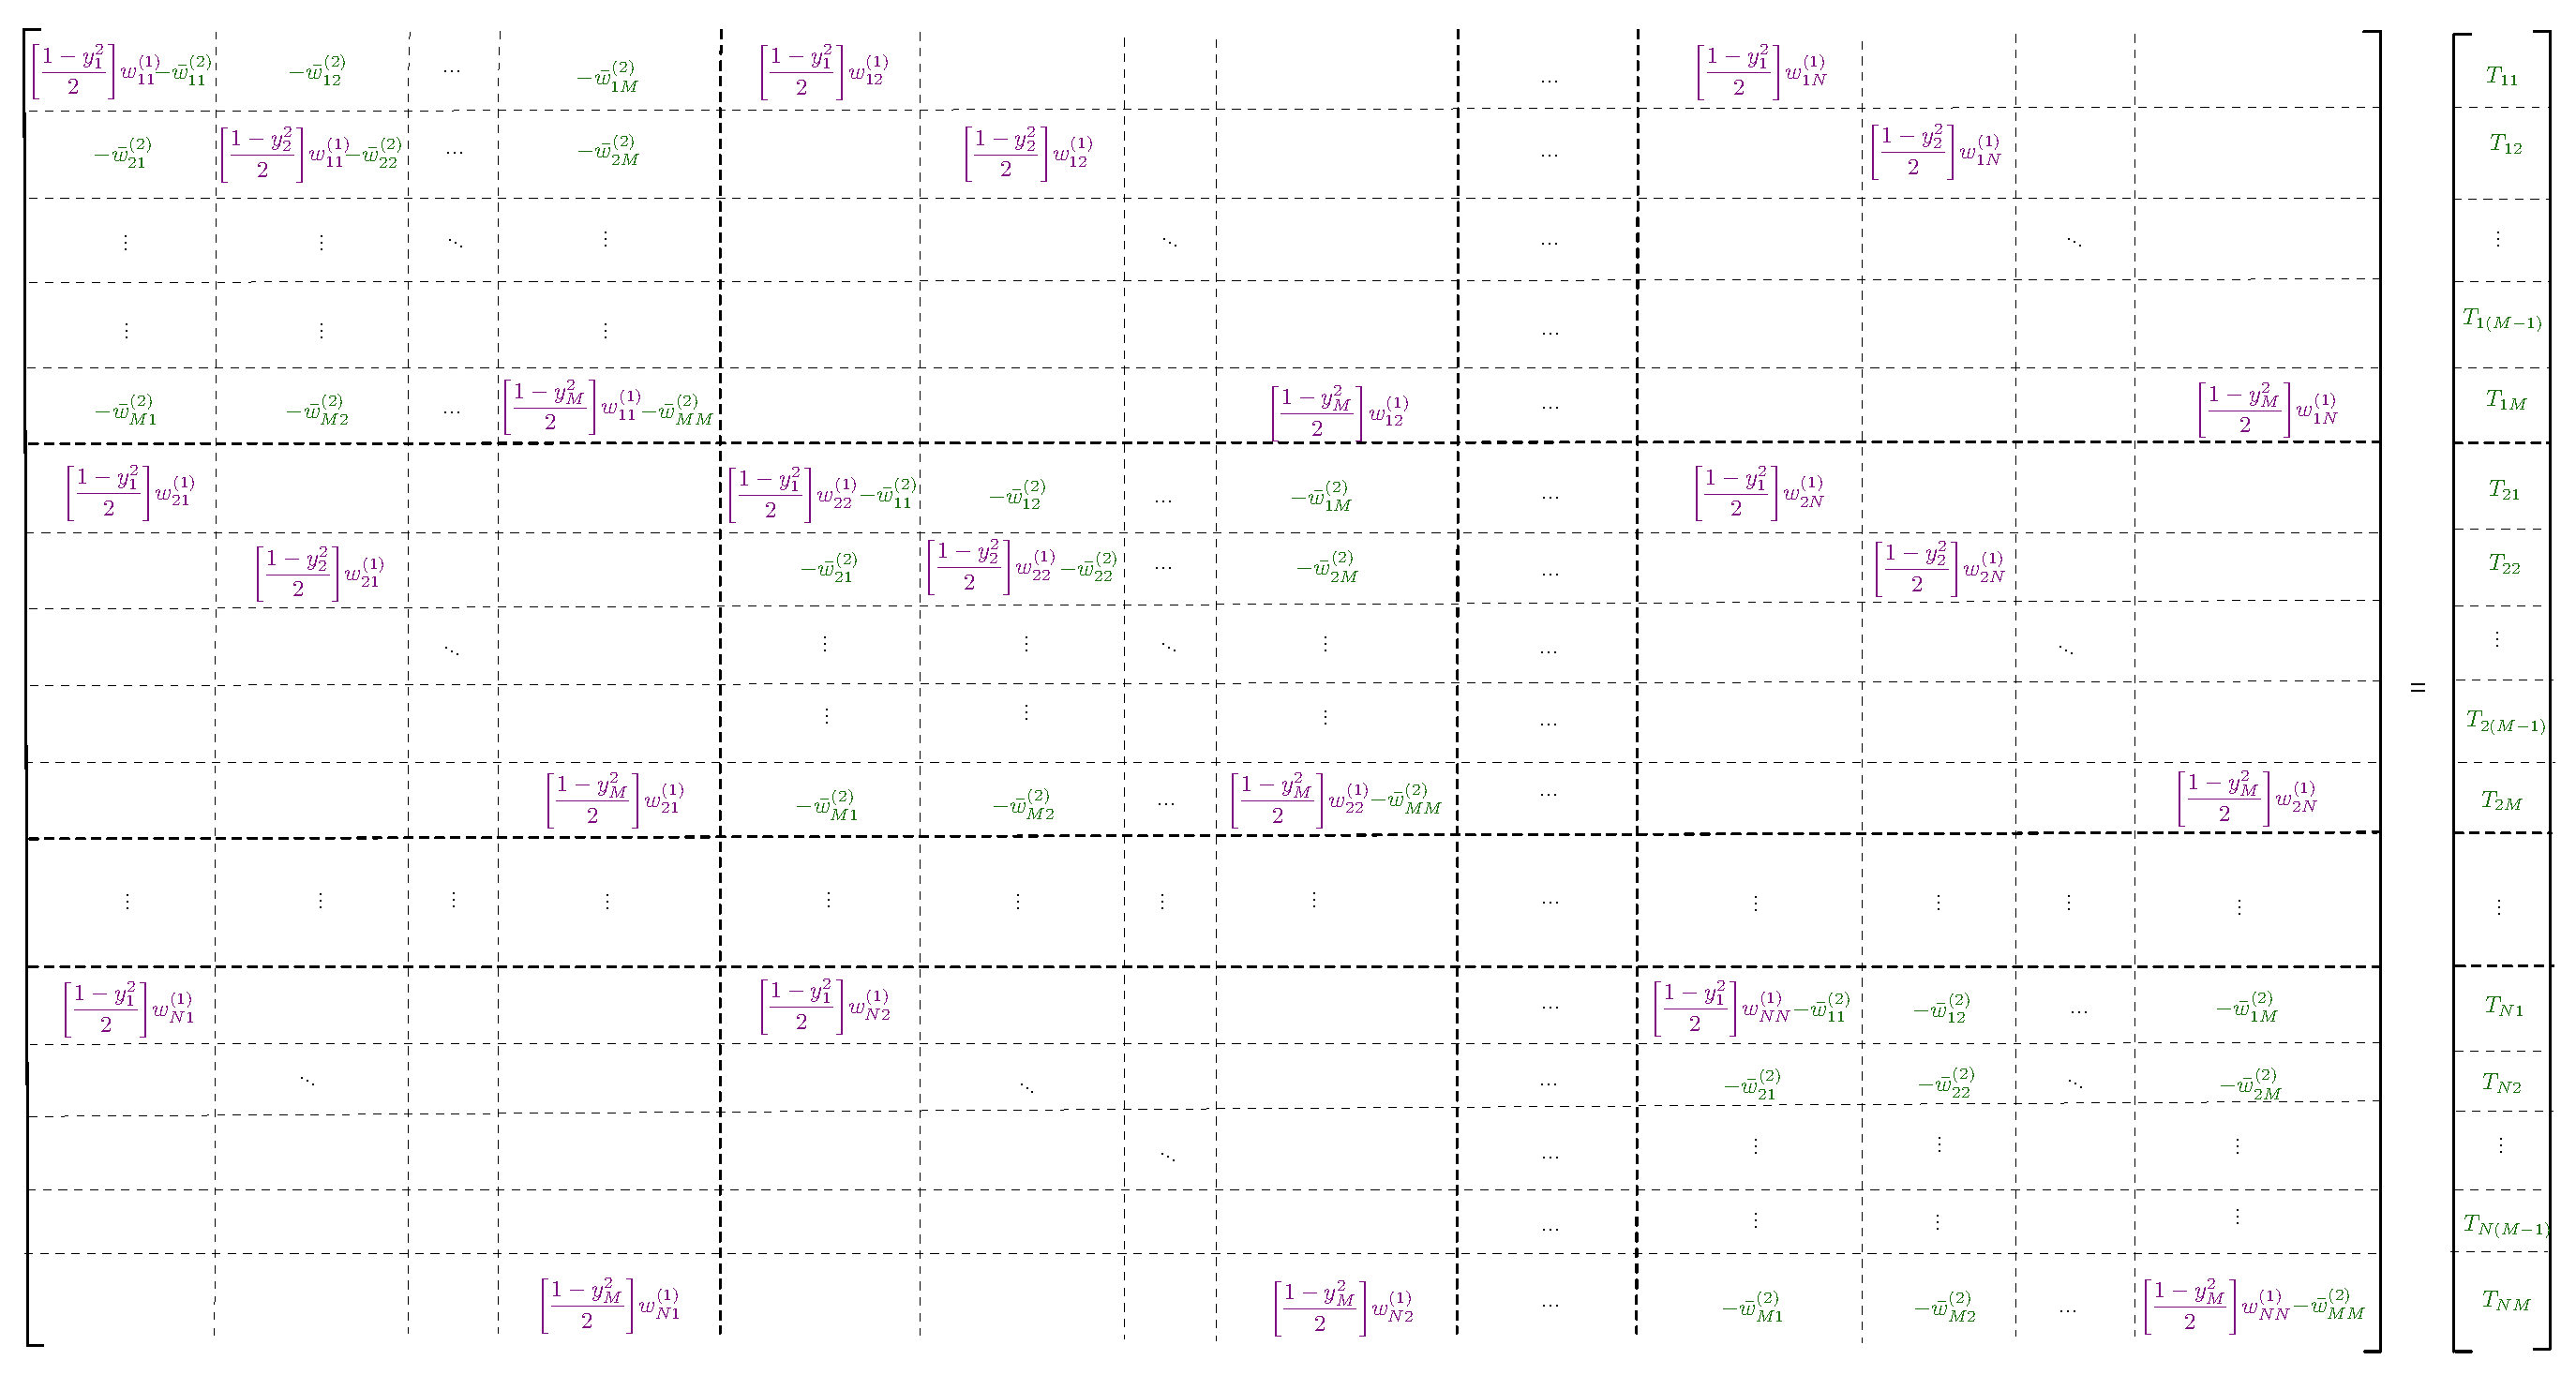
\includegraphics[width=22cm]{figures/matrixGiantErasedEq}    % The printed column width is 8.4 cm.
\vspace*{6mm}
\caption{Matrix representation of the system of equations.} 
\label{matrixGiantErasedEq}
\end{center}
\end{figure}
\end{landscape}

\begin{landscape}
\thispagestyle{empty}
\begin{figure}
\begin{center}
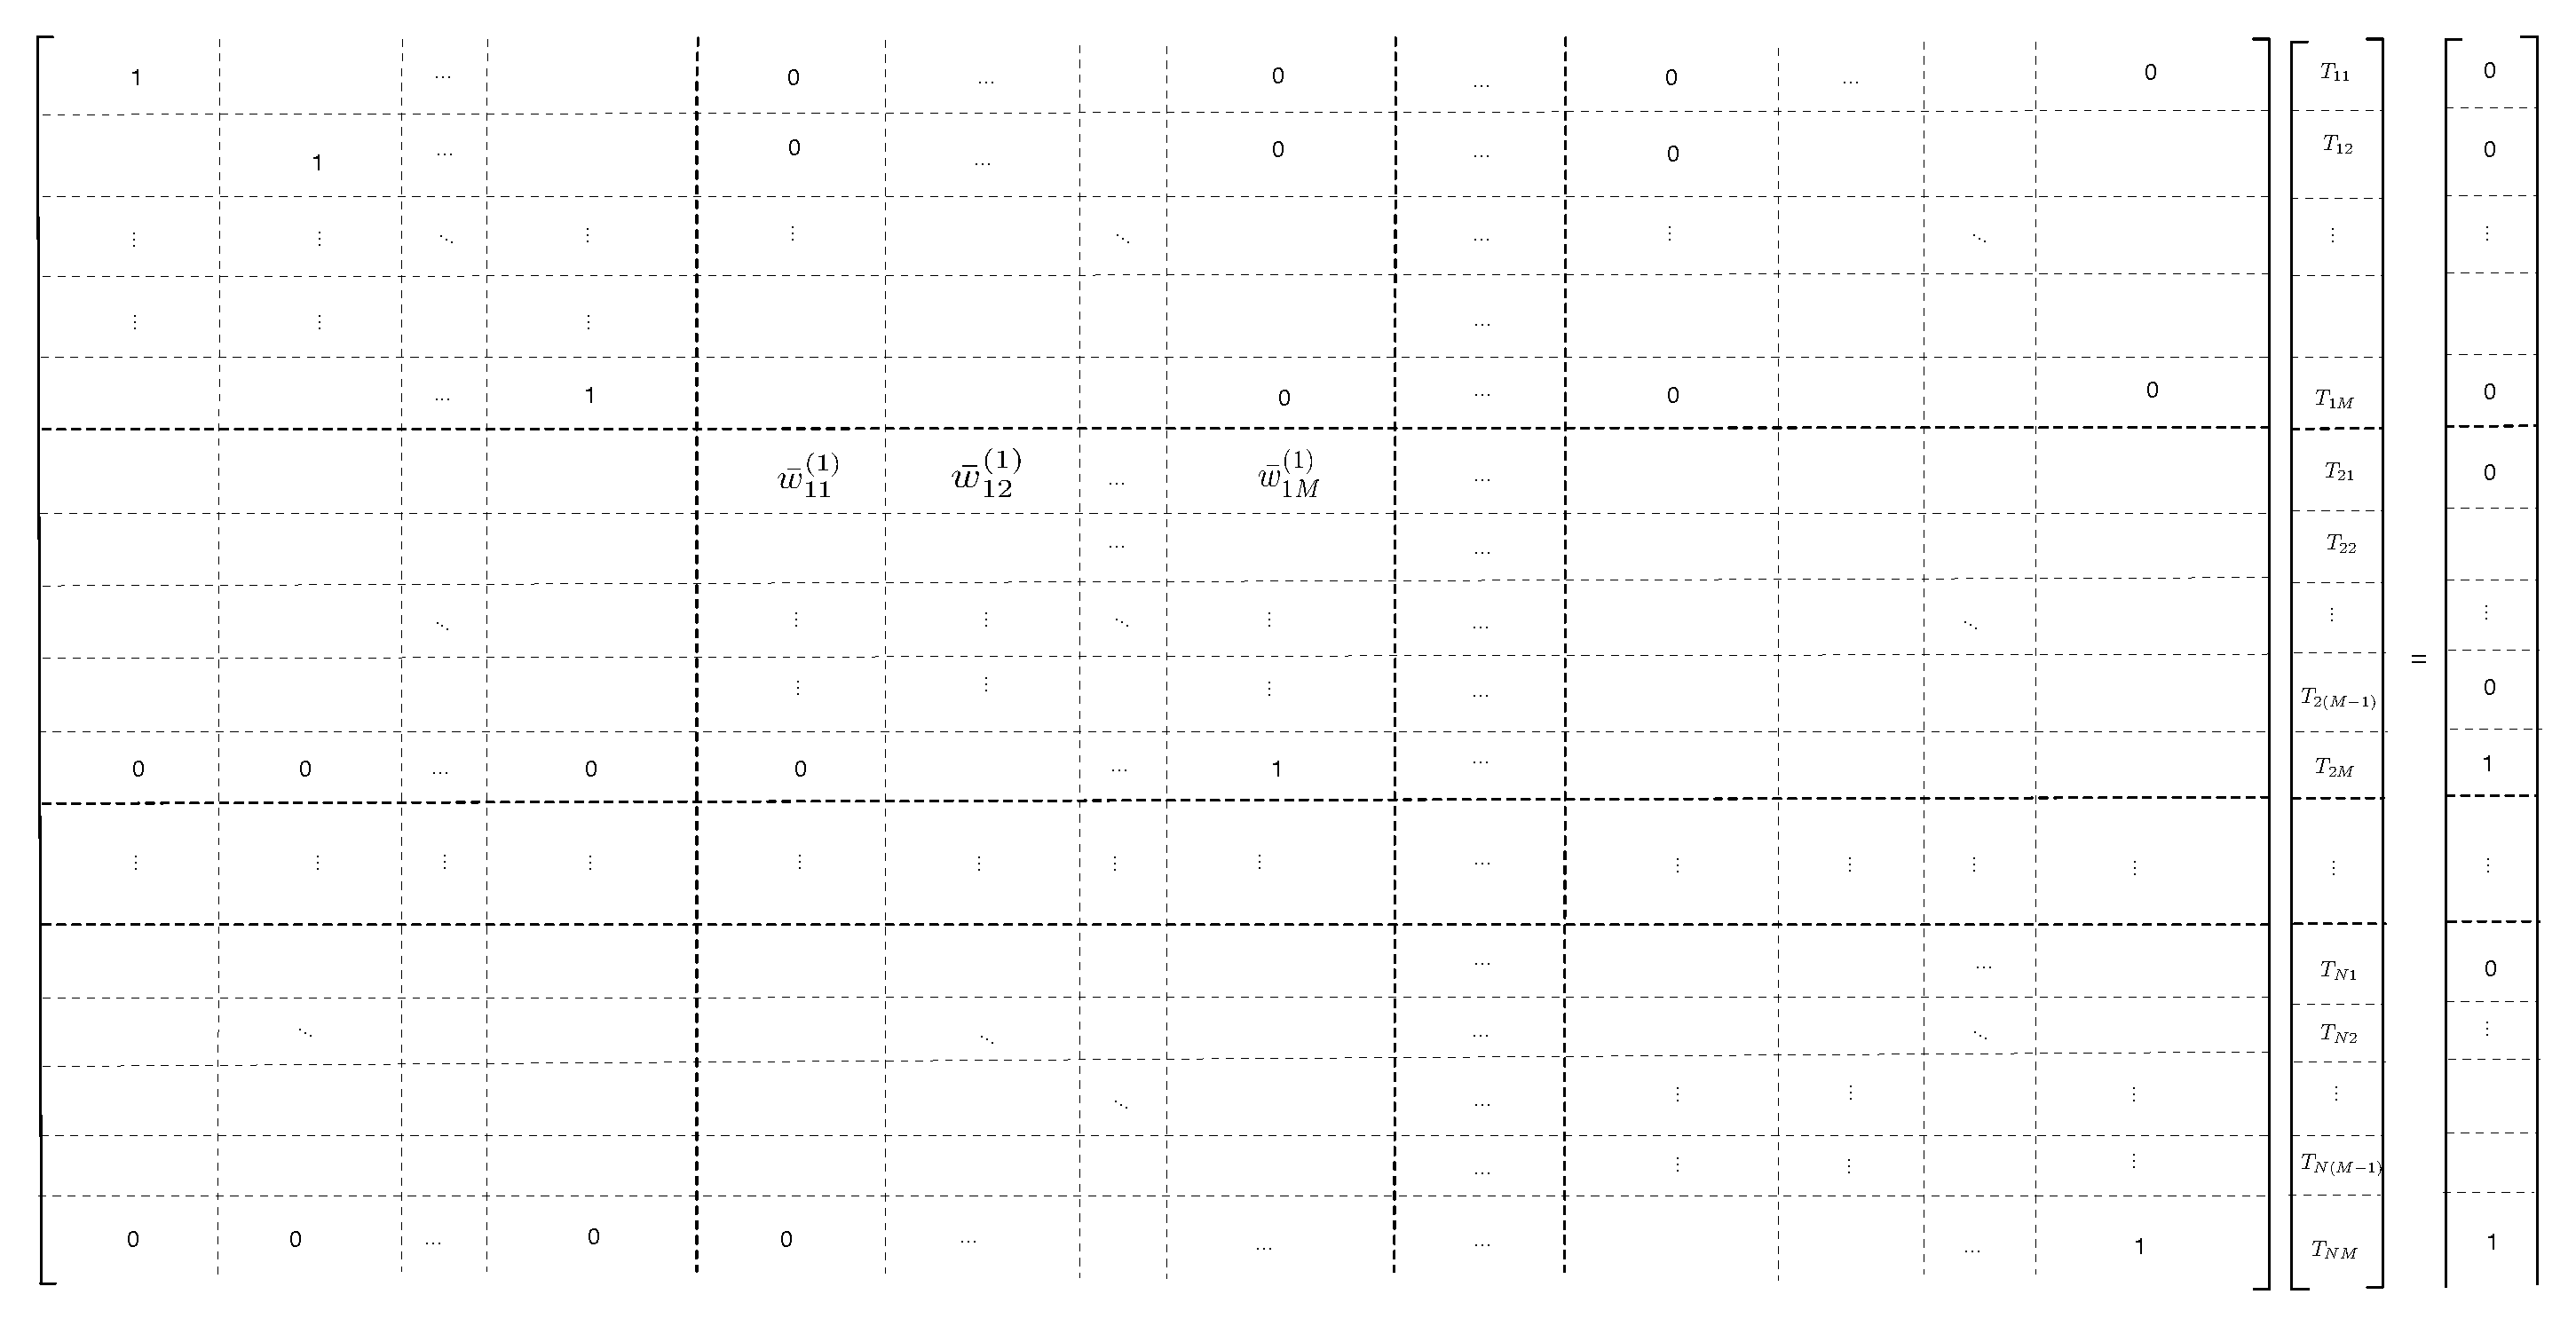
\includegraphics[width=22cm]{figures/matrixBoundaries}    % The printed column width is 8.4 cm.
\vspace*{6mm}
\caption{Rows to update in the system of equations due to boundary conditions.} 
\label{matrixBoundaries}
\end{center}
\end{figure}
\end{landscape}

\subsection*{Newton-Raphson Method}

Newton-Raphson method is used for finding successively better approximations to the roots of a real-valued function. This method can be implemented for higher dimensions, at which there are several functions of several variables.  Newton-Raphson method for higher dimension is given in Eqn.\eqref{matrixForm}.

\begin{equation} \label{matrixForm}
\mathbf{x}_{k+1}=\mathbf{x}_{k}-\mathbf{J}^{-1}\mathbf{y}_{k}
\end{equation}


where $\mathbf{x}=[x_1;\text{ }x_2;\text{ }\dots;\text{ }x_n]$ and $\mathbf{y}=[y_1;\text{ }y_2;\text{ }\dots;\text{ }y_n]$. $\mathbf{J}$ is the Jacobian matrix and it is given \eqref{jacobian}.


\begin{equation} \label{jacobian}
\mathbf{J}=
\begin{bmatrix}
\frac{\partial f_1}{\partial x_1} &
\frac{\partial f_1}{\partial x_2} &
\dots &
\frac{\partial f_1}{\partial x_n} \\[0.4em]
\frac{\partial f_2}{\partial x_1} &
\frac{\partial f_2}{\partial x_2} &
\dots &
\frac{\partial f_2}{\partial x_n} \\[0.2em]
\vdots &
\vdots &
\ddots &
\vdots \\[0.2em]
\frac{\partial f_n}{\partial x_1} &
\frac{\partial f_n}{\partial x_2} &
\dots &
\frac{\partial f_n}{\partial x_n}
\end{bmatrix}
\end{equation}
